\chapter{ЗАГРУЗКА МОДЕЛЕЙ СЦЕН И ОБЪЕКТОВ ОКРУЖЕНИЯ В ФОРМАТАХ SDF И STL}
\label{cha:sdf}

\section{Постановка задачи}

Помимо моделей роботов, для проведения виртуального эксперимента необходимо
описание рабочей сцены: статического окружения, препятствий, объектов
манипулирования. Для этого применяются форматы:
\begin{itemize}
  \item \textbf{SDF} (Simulation Description Format)~\cite{sdformat} ---
        основанный на XML формат описания сцены (мир, модели, звенья, суставы, источники света, физические
        свойства); фактический стандарт в экосистеме Gazebo;
  \item \textbf{STL} (STereoLithography) --- формат хранения полигональной
        (треугольной) сетки, широко используемый для представления геометрии
        деталей и препятствий.
\end{itemize}

Задача --- реализовать загрузку сцен SDF и геометрии STL и их отображение в той
же трёхмерной сцене, что и модели роботов. Работа выполнена в репозитории
\texttt{modeuler} (модуль \texttt{scene}, компоненты \texttt{utils/scene\_loader},
\texttt{utils/model\_loader}, \texttt{utils/scene\_manager}).

\section{Загрузка сцен SDF}

Разбор SDF выполняется аналогично URDF: дерево XML обходится с извлечением
вложенных моделей, звеньев и их геометрии; для каждой модели строится локальная
система координат, а модели размещаются в мировой системе согласно заданным
позам (\texttt{pose}). Поскольку SDF и URDF имеют близкую объектную модель
(звенья, суставы, геометрия, позы), в \texttt{modeuler} они приводятся к единому
внутреннему представлению сцены (\texttt{scene.hpp}), что позволяет переиспользовать
конвейер отрисовки и подсистему управления камерой.

\section{Загрузка геометрии STL}

Загрузка STL реализована через vsgXchange: бинарные и текстовые STL-файлы
преобразуются в узлы графа сцены с буферами вершин и нормалей. Для отсутствующих
нормалей выполняется их восстановление по граням. Загруженная сетка
присоединяется к узлу соответствующего объекта сцены и далее обрабатывается
конвейером отрисовки наравне с прочей геометрией.

\begin{figure}[ht]
  \centering
  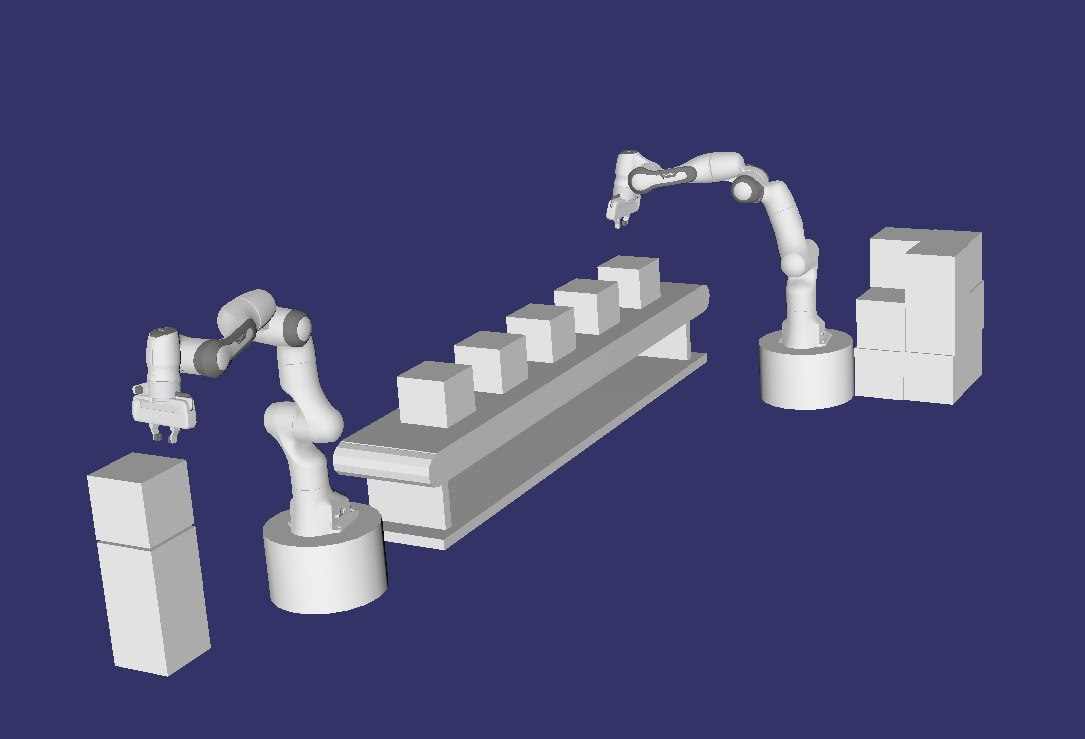
\includegraphics[width=0.9\textwidth]{figures/modeuler-scene.jpg}
  \caption{Загруженная рабочая сцена: конвейерная линия с двумя манипуляторами
    и объектами окружения}
  \label{fig:sdf-scene}
\end{figure}

Пример загруженной сцены показан на рисунке~\ref{fig:sdf-scene}: рабочая ячейка
с конвейерной линией, двумя манипуляторами и объектами манипулирования;
статическое окружение и полигональная геометрия объектов импортированы из
описания сцены и отображаются совместно с моделями роботов.

\section{Результаты}

Реализованы модуль загрузки сцен в формате SDF и модуль импорта полигональной
геометрии в формате STL. Оба источника приводятся к единому внутреннему
представлению сцены и визуализируются совместно с моделями роботов. Загрузка
проверена на наборе тестовых сцен; объекты размещаются в соответствии с
заданными в SDF позами, геометрия STL отображается без искажений.
